\documentclass[12pt, twoside]{report}
\usepackage{libertine}

% General packages:
\usepackage[utf8]{inputenc}    % Input encoding
\usepackage[T1]{fontenc}       % Font encoding
\usepackage[british]{babel}    % Naming of figures and such
\usepackage[british]{isodate}  % Formatting of dates
\cleanlookdateon               % Show dates cleanly.
%\usepackage{xurl}              % Allow line breaks anywhere in URLs.
\usepackage{minted}            % Needs to be loaded before `csquotes`.
\usepackage[
    citestyle    = authoryear,
    bibstyle     = authoryear,
    giveninits   = true,
    uniquename   = init,
    uniquelist   = false,
    sortlocale   = en_GB,
    backend      = biber,
    backref      = true,
    maxbibnames  = 100,
    maxcitenames = 1,
    dashed       = false,
    % Needed to get sorting right for tussenvoegsels.
    %sortcites    = true,       
    ]{biblatex}                % Bibliography
\usepackage[
    style=american
    ]{csquotes}                % Required for BiBLaTeX
\usepackage{import}            % Importing subdocuments
\usepackage{standalone}        % Compilable subdocuments
% `setspace` needs to be loaded before `hyperref`.
\usepackage{setspace}          % Set line spacing
\usepackage{hyperref}          % Clickable references
\usepackage{microtype}         % Nice typography
\usepackage{makeidx}           % Make an index
\usepackage{silence}           % Silence warnings and errors
\WarningFilter{remreset}{The remreset package}
\WarningFilter*[parskip]{latex}{Command}

% Set line spacing.
\setstretch{1.25}

% Page layout:
\usepackage{tocloft}         % Control ToC
\usepackage[
    a4paper,
    bottom     = 1.1in,
    top        = 1.1in,
    left       = 1.1in,
    right      = 1.1in,
    headheight = 15pt,
    footskip   = 1.5\baselineskip
    ]{geometry}              % Margins
\usepackage{fancyhdr}        % Header
\usepackage{lastpage}        % Page numbers in footer
\usepackage{setspace}        % Line spacing
\usepackage{ragged2e}        % Better line endings
\ActivateWarningFilters[parskip]
\usepackage[
    parfill
    ]{parskip}               % Newlines instead of indentation
\DeactivateWarningFilters[parskip]
\usepackage{titlesec}        % Size of sections
\usepackage{titlecaps}       % Automatic capitalisation of titles
\usepackage[
    hang,
    bottom
    ]{footmisc}              % Configure footnotes
\usepackage{afterpage}       % Include stuff after the current page
\usepackage{placeins}        % Things like `\FloatBarrier`
\usepackage{pdflscape}       % Turn pages sideways
\usepackage{emptypage}       % Remove pagenumbers on empty pages

% Utility:
\usepackage[table]{xcolor}   % Colours
\usepackage[
    separate-uncertainty=true,
    per-mode=symbol
    ]{siunitx}               % Display units
\usepackage{enumitem}        % Better enumeration
\usepackage{xifthen}         % If statements
\usepackage{xpatch}          % Patch things
\usepackage{lipsum}          % Dummy text
\usepackage{listings}        % Listings
\usepackage{xparse}          % Better arguments for \newcommand
\usepackage{xfrac}           % Better fractions
\usepackage{etoolbox}        % Patch stuff
\usepackage[
    notquote
    ]{hanging}               % Hanging paragraphs
\usepackage{scalerel}        % Scale objects
\usepackage{soul}            % Highlighting

% Figures:
\usepackage{pgfplots}        % Plots
\pgfplotsset{compat=newest}
\usepackage{tikz}            % TikZ figures
\usepackage{float}           % Control floating of figures
\usepackage{multirow}        % Cells spanning multiple rows
\usepackage{graphicx}        % Graphics
\usepackage{caption}         % Subfigures and captions
\usepackage{subcaption}      % Subfigures and captions
\usepackage{booktabs}        % Nice looking tables
\usepackage{tabularx}        % Extended functionality for tables

% Math:
\usepackage{amsmath}         % Math
\usepackage{amssymb}         % Math symbols
\usepackage{mathtools}       % Math tools
\usepackage{amsthm}          % Theorems
\usepackage{thmtools}        % More math theorems
\usepackage{bm}              % Bold math symbols
\usepackage{bbm}             % More bold math symbols
\usepackage{cancel}          % Cancel equations
\usepackage{upgreek}         % Upright greek symbols
\usepackage[
    artemisia
    ]{textgreek}             % Greek symbols in text

% This package should be loaded last.
\usepackage[
    noabbrev,
    capitalize,
    nameinlink]{cleveref}    % Automatic referencing

% Add a comma in the cite style.
\renewcommand*{\nameyeardelim}{\addcomma\space}

% Make sure that every `\citeyear` also prints the disambiguating `extradate`.
\DeclareCiteCommand{\citeyearlabel}
    {\usebibmacro{prenote}}
    {\printfield{year}\printfield{extradate}}
    {\multicitedelim}
    {\usebibmacro{postnote}}
\let\citeyearold\citeyear
\let\citeyear\citeyearlabel
\let\citeyearnolabel\citeyearold

% Define a standard for citing within theorem statements.
\newcommand{\theoremcite}[1]{\citeauthor{#1}, \citeyear{#1}}

\newcommand{\fulltextcite}[1]{%
    \AtNextCite{\AtEachCitekey{\defcounter{maxnames}{999}}}%
    \textcite{#1}%
}
\newcommand{\fullparencite}[1]{%
    \AtNextCite{\AtEachCitekey{\defcounter{maxnames}{999}}}%
    \parencite{#1}%
}

% Remove the colon after "In" in the bibliograhpy.
\renewbibmacro*{in:}{\bibstring{in} }

% Tune the electronic print field.
\DeclareFieldFormat{eprint}{%
  \iffieldundef{eprinttype}
    {Electronic print}
    {\thefield{eprinttype}}%
  \addcolon\space
  \ifhyperref
    {\url{#1}}
    {\nolinkurl{#1}}%
  \iffieldundef{eprintclass}
    {}
    {\addspace\mkbibparens{\thefield{eprintclass}}}\printtext{.}}

% Tune URL.
\DeclareFieldFormat{url}{\mkbibacro{URL}\addcolon\space\url{#1}\printtext{.}}

% Tune DOI.
\DeclareFieldFormat{doi}{%
  \mkbibacro{DOI}\addcolon\space
  \ifhyperref
    {\href{https://doi.org/#1}{\nolinkurl{#1}}}
    {\nolinkurl{#1}}\printtext{.}}

% In the below, we will redefine `\finentry` to not print a period if
%` pageref` exists. The period is then added back by `pageref`, but before the
% parentheses. Problems occur when `urldate` is also defined. In that case, 
% the extra period by `pageref` will add a period after `urldate`s
% parentheses, which we do not want. We use the toggle `printperiod` to detect
% this case.

% Tune "visited on".
\DeclareFieldFormat{urldate}{\mkbibparens{\bibstring{urlseen}\space#1\printtext{.}}}
\newtoggle{printperiod}
\toggletrue{printperiod}
\AtBeginBibliography{\renewbibmacro*{urldate}{\printurldate\togglefalse{printperiod}}}

% Tune "cited on".
\renewbibmacro*{finentry}{\iflistundef{pageref}{}{\renewcommand{\finentrypunct}{}}\finentry}
\renewbibmacro*{pageref}{%
  \iflistundef{pageref}
    {}
    {\iftoggle{printperiod}{\setunit{\adddot\addspace}}{}\toggletrue{printperiod}\printtext[parens]{%
       \ifnumgreater{\value{pageref}}{1}
         {\bibstring{backrefpages}\ppspace}
         {\bibstring{backrefpage}\ppspace}%
          \printlist[pageref][-\value{listtotal}]{pageref}.}}}

% Add Oxford comma.
\DefineBibliographyExtras{british}{\def\finalandcomma{\addcomma}}

% Don't abbreviate the backreferences.
\DefineBibliographyStrings{english}{%
    backrefpage = {Cited on page},
    backrefpages = {Cited on pages}
}

% Get tussenvoegsels right. This is not a perfect solution, because the
% in-text citations will be sorted as if the tussenvoegsel is part of the
% last name.
\makeatletter
\AtBeginDocument{\toggletrue{blx@useprefix}}
\AtBeginBibliography{\togglefalse{blx@useprefix}}
\makeatother

% Make an index.
\makeindex

% Show the page number in the bottom center.
\fancypagestyle{plain}{
    \fancyhf{}                          % Clear all header and footers.
    \renewcommand{\headrulewidth}{0pt}  % Remove the header rule.
    \cfoot{\thepage}                    % Show page number in the center.
}
\pagestyle{plain}

% Chapter styling from https://texblog.org/2012/07/03/fancy-latex-chapter-styles/
\newcommand{\hsp}{\hspace{20pt}}
\titleformat{\chapter}[hang]
    {\Huge\bfseries}
    {\thechapter\hsp\textcolor{gray75}{|}\hsp}
    {0pt}
    {\Huge\bfseries}
\titleformat{\section}
    {\normalfont\Large\bfseries\raggedright}
    {\thesection}
    {1em}
    {}
\titleformat{\subsection}
    {\normalfont\large\bfseries\raggedright}
    {\thesubsection}
    {1em}
    {}

% Set spacing after chapter equal to spacing right before section. Then
% things look nicely aligned.
\titlespacing{\chapter}{0pt}{3.5ex}{3.5ex}

% Define the styling of paragraphs.
\renewcommand{\paragraph}[1]{\textbf{#1.}}

% Redefine abstract environment.
\renewenvironment{abstract}
    {\begingroup
    \setstretch{1.25}
    \begin{center}
        \textbf{Abstract}
    \end{center}}
    {\par
    \endgroup}

% Kill any use of the \cite command.
\renewcommand{\cite}[1]{\PackageError{thesis}{use either parencite or authorcite}{}}

% Configure captions.
\WarningFilter{caption}{Unused \captionsetup}
\captionsetup[table]{font=small}
\captionsetup[figure]{font=small}

% Shortcuts for writing.
\newcommand{\ie}{\textit{i.e.}}
\newcommand{\Ie}{\textit{I.e.}}
\newcommand{\eg}{\textit{e.g.}}
\newcommand{\Eg}{\textit{E.g.}}
\newcommand{\cf}{\textit{c.f.}}
\newcommand{\Cf}{\textit{C.f.}}

% \ifempty command:
\newcommand{\ifempty}[3]{\ifthenelse{\equal{#1}{}}{#2}{#3}}

% Style footnotes.
\setlength{\skip\footins}{\baselineskip}
\setlength{\footnotesep}{.75\baselineskip}
\renewcommand{\footnotelayout}{\setstretch{1.0}}
\setlength{\footnotemargin}{1em}

% Typewriter font:
\renewcommand*{\ttdefault}{pcr}  % Courier
\newcommand{\code}[1]{{\small\texttt{#1}}}

% Define some colours.
\definecolor{darkblue} {rgb} {0.0 , 0.0 , 0.65}
\definecolor{darkred}  {rgb} {0.80, 0.0 , 0.0 }
\definecolor{redaccent}{HTML}{E64C66}
\definecolor{darkgreen}{rgb} {0.0 , 0.50, 0.0 }
\definecolor{gray75}   {gray}{0.75}

% Define shortcuts for colours.
\newcommand{\red}[1]{{\color{red} #1}}
\newcommand{\blue}[1]{{\color{blue} #1}}
\newcommand{\green}[1]{{\color{green} #1}}
\newcommand{\orange}[1]{{\color{orange} #1}}
\newcommand{\darkred}[1]{{\color{darkred} #1}}
\newcommand{\darkblue}[1]{{\color{darkblue} #1}}
\newcommand{\darkgreen}[1]{{\color{darkgreen} #1}}
\newcommand{\magenta}[1]{{\color{magenta} #1}}
\newcommand{\grey}[1]{{\color{gray} #1}}

% Use colours to define checkmarks and crosses.
\usepackage{pifont}
\newcommand{\xmark}{\text{\ding{55}}}
\newcommand{\cmark}{\text{\ding{51}}}
\newcommand{\good}{\darkgreen{$\checkmark$}}
\newcommand{\mediumgood}{\orange{$\checkmark$}}
\newcommand{\mediumbad}{\orange{\xmark}}
\newcommand{\bad}{\darkred{\xmark}}

% Load TikZ libraries.
\usetikzlibrary{
    calc,
    positioning,
    fit,
    tikzmark,
    arrows.meta,
    shapes,
    decorations.pathreplacing,
    intersections,
    through
}
% Graphical models:
\tikzset{
    line/.style = {
        thick,
        ->,
        > = {
            Triangle[length=1.5mm, width=1.5mm]
        }
    },
    arrow/.style = {
        line
    },
    % Invisible node:
    hidden node/.style = {
        circle,
        minimum size = 1cm,
        draw = white,
        thick
    },
    % Latent variable:
    latent node/.style = {
        hidden node,
        draw = black,
    },
    % Latent variable:
    factor node/.style = {
        hidden node,
        rectangle,
        draw = black,
    },
    % Observed variable:
    observed node/.style = {
        latent node,
        fill = gray!15
    },
    % Plate:
    plate/.style = {
        draw,
        label={[anchor=north west]south west:#1},
        rounded corners=2pt,
        shape=rectangle,
        inner sep=10pt,
        thick
    }
}

% Circled number:
\newcommand{\ballnumber}[1]{%
    \tikz[baseline=(n.base)] \node[circle,fill=.,inner sep=1pt,text=white] (n) {\normalshape\bfseries\footnotesize #1};%
}
\newcommand{\itemballnumber}[1]{%
    \raisebox{.5pt}{\ballnumber{#1}}%
}

% Style enumerate and lists. Do not use `label=(\arabic*)` because equation
% numbering already uses the same style.
\setenumerate{topsep=.25\baselineskip, itemsep=0pt}
\setlist{topsep=.25\baselineskip, itemsep=0pt}
% \setlist[enumerate]{
%     label=(\arabic*),
%     itemsep=-0.25\baselineskip,
%     topsep=0.25\baselineskip,
%     after={\vspace*{0.25\baselineskip}}
% }
% \setlist[enumerate,2]{
%     topsep=-0.25\baselineskip,
%     itemsep=0pt,
%     label=(\alph*)
% }
% \setlist[enumerate,3]{
%     topsep=-0.25\baselineskip,
%     itemsep=0pt,
%     label=(\roman*)
% }
% \setlist[itemize]{
%     label=\textbullet,
%     itemsep=-0.25\baselineskip,
%     topsep=0.25\baselineskip
% }
% \setlist[itemize,2]{
%     topsep=-0.25\baselineskip,
%     itemsep=0pt
% }
% \setlist[itemize,3]{
%     topsep=-0.25\baselineskip,
%     itemsep=0pt
% }

% Set the default float placement correctly.
\floatplacement{figure}{tbp}
\floatplacement{table}{tbp}

% Set spacing between figures and text.
\setlength{\textfloatsep}{30pt plus 1.0pt minus 2.0pt}
\setlength{\floatsep}{30pt plus 1.0pt minus 2.0pt}
\setlength{\intextsep}{30pt plus 1.0pt minus 2.0pt}

% Adjust line spacing in captions.
\captionsetup{font={stretch=1.25}}

% Newline for in a title.
\newcommand{\tnl}{\texorpdfstring{\\}{}}

% Define outline tools.
\newcommand{\outline}[1]{
    \parbox{\linewidth}{
        \setstretch{1.0}
        \color{darkgreen}
        #1
    }\vspace{\parskip}
}
\newlist{outlinelist}{enumerate}{1}
\setlist[outlinelist]{
    label=\arabic*.,
    noitemsep,
    topsep=0pt,
    parsep=0pt,
    partopsep=0pt
}
\newcommand{\note}[1]{{\color{darkred}#1}}

% Left-justified text in tabularx environment:
\newcolumntype{L}{>{\RaggedRight\arraybackslash}X}

% Hyperlink setup.
\hypersetup{
    colorlinks,
    citecolor = black,
    filecolor = black,
    linkcolor = black,
    urlcolor  = black
}

% Landscape figures:
\newcommand{\landscapefloat}[1]{
    \afterpage{
        \begin{landscape}
            #1
        \end{landscape}
    }
}

% Hanging full citation:
\newcommand{\hangcite}[1]{\hangpara{\bibhang}{1}\AtNextCite{\defcounter{maxnames}{99}}\fullcite{#1}}

% Define \charfusion. From https://tex.stackexchange.com/a/52673.
\makeatletter
\def\moverlay{\mathpalette\mov@rlay}
\def\mov@rlay#1#2{\leavevmode\vtop{%
   \baselineskip\z@skip \lineskiplimit-\maxdimen
   \ialign{\hfil$\m@th#1##$\hfil\cr#2\crcr}}}
    \newcommand{\charfusion}[3][\mathord]{
        #1{\ifx#1\mathop\vphantom{#2}\fi
        \mathpalette\mov@rlay{#2\cr#3}}
        \ifx#1\mathop\expandafter\displaylimits\fi
    }
\makeatother

% Sha symbol.
%   Source: https://tex.stackexchange.com/questions/124738/i-just-want-to-write-sha-without-ruining-everything
\DeclareFontFamily{U}{wncy}{}
\DeclareFontShape{U}{wncy}{m}{n}{<->wncyr10}{}
\DeclareSymbolFont{mcy}{U}{wncy}{m}{n}
\DeclareMathSymbol{\Sha}{\mathord}{mcy}{"58}

% Define a bigger \cdot.
%   Source: https://tex.stackexchange.com/questions/235118/making-a-thicker-cdot-for-dot-product-that-is-thinner-than-bullet
\makeatletter
\newcommand*\bigcdot{\mathpalette\bigcdot@{.5}}
\newcommand*\bigcdot@[2]{\mathbin{\vcenter{\hbox{\scalebox{#2}{$\m@th#1\bullet$}}}}}
\makeatother

% Bold math symbols from text greeks:
\newcommand{\mathbfup}[1]{\mathord{\textnormal{\textbf{#1}}}}

% Bold characters:
\renewcommand{\vec}[1]{\boldsymbol{#1}}
\newcommand{\vecu}[1]{\hat{\vec{#1}}}
\newcommand{\mat}[1]{\vec{#1}}

% Predefined matrices and vectors:
\newcommand{\vnull}{\mathbf{0}}

\newcommand{\va}{\mathbf{a}}
\newcommand{\vb}{\mathbf{b}}
\newcommand{\vc}{\mathbf{c}}
\newcommand{\vd}{\mathbf{d}}
\newcommand{\ve}{\mathbf{e}}
\newcommand{\vf}{\mathbf{f}}
\newcommand{\vg}{\mathbf{g}}
\newcommand{\vh}{\mathbf{h}}
\newcommand{\vi}{\mathbf{i}}
\newcommand{\vj}{\mathbf{j}}
\newcommand{\vk}{\mathbf{k}}
\newcommand{\vl}{\mathbf{l}}
\newcommand{\vm}{\mathbf{m}}
\newcommand{\vn}{\mathbf{n}}
\newcommand{\vo}{\mathbf{o}}
\newcommand{\vp}{\mathbf{p}}
\newcommand{\vq}{\mathbf{q}}
\newcommand{\vr}{\mathbf{r}}
\newcommand{\vs}{\mathbf{s}}
\newcommand{\vt}{\mathbf{t}}
\newcommand{\vu}{\mathbf{u}}
\newcommand{\vv}{\mathbf{v}}
\newcommand{\vw}{\mathbf{w}}
\newcommand{\vx}{\mathbf{x}}
\newcommand{\vy}{\mathbf{y}}
\newcommand{\vz}{\mathbf{z}}

% Must be enclosed in another group.
\newcommand{\vmu}{{\mathbfup{\textmu}}}
\newcommand{\vtheta}{{\bm{\uptheta}}}
\newcommand{\vphi}{{\mathbfup{\textphi}}}
\newcommand{\vtau}{{\mathbfup{\texttau}}}
\newcommand{\vep}{{\mathbfup{\textepsilon}}}
\newcommand{\vth}{{\mathbfup{\texttheta}}}

\newcommand{\mA}{\mathbf{A}}
\newcommand{\mB}{\mathbf{B}}
\newcommand{\mC}{\mathbf{C}}
\newcommand{\mD}{\mathbf{D}}
\newcommand{\mE}{\mathbf{E}}
\newcommand{\mF}{\mathbf{F}}
\newcommand{\mG}{\mathbf{G}}
\newcommand{\mH}{\mathbf{H}}
\newcommand{\mI}{\mathbf{I}}
\newcommand{\mJ}{\mathbf{J}}
\newcommand{\mK}{\mathbf{K}}
\newcommand{\mL}{\mathbf{L}}
\newcommand{\mM}{\mathbf{M}}
\newcommand{\mN}{\mathbf{N}}
\newcommand{\mO}{\mathbf{O}}
\newcommand{\mP}{\mathbf{P}}
\newcommand{\mQ}{\mathbf{Q}}
\newcommand{\mR}{\mathbf{R}}
\newcommand{\mS}{\mathbf{S}}
\newcommand{\mT}{\mathbf{T}}
\newcommand{\mU}{\mathbf{U}}
\newcommand{\mV}{\mathbf{V}}
\newcommand{\mW}{\mathbf{W}}
\newcommand{\mX}{\mathbf{X}}
\newcommand{\mY}{\mathbf{Y}}
\newcommand{\mZ}{\mathbf{Z}}

\newcommand{\mSigma}{\mathbfup{\textSigma}}

% Letters commonly used in blackboard bold font:
\newcommand{\Ab}{\mathbb{A}}
\newcommand{\Bb}{\mathbb{B}}
\newcommand{\Db}{\mathbb{D}}
\newcommand{\C}{\mathbb{C}}
\newcommand{\E}{\mathbb{E}}
\newcommand{\Hb}{\mathbb{H}}
\newcommand{\Jb}{\mathbb{J}}
\newcommand{\K}{\mathbb{K}}
\newcommand{\Lb}{\mathbb{L}}
\newcommand{\Mb}{\mathbb{M}}
\newcommand{\N}{\mathbb{N}}
\renewcommand{\P}{\mathbb{P}}
\newcommand{\Q}{\mathbb{Q}}
\newcommand{\R}{\mathbb{R}}
\newcommand{\eR}{\overline{\mathbb{R}}}
\newcommand{\Sb}{\mathbb{S}}
\newcommand{\Tb}{\mathbb{T}}
\newcommand{\V}{\mathbb{V}}
\newcommand{\Z}{\mathbb{Z}}

% Letters commonly used in calligraphic font:
\newcommand{\A}{\mathcal{A}}
\newcommand{\B}{\mathcal{B}}
\newcommand{\Cc}{\mathcal{C}}
\newcommand{\D}{\mathcal{D}}
\newcommand{\Ec}{\mathcal{E}}
\newcommand{\F}{\mathcal{F}}
\newcommand{\G}{\mathcal{G}}
\let\Haccent\H
\renewcommand{\H}{\mathcal{H}}
\newcommand{\J}{\mathcal{J}}
\newcommand{\Jrat}{\mathcal{J}_{\text{rat}}}
\newcommand{\Kc}{\mathcal{K}}
\renewcommand{\L}{\mathcal{L}}
\newcommand{\Li}{\mathcal{L}{}^1}
\newcommand{\eLi}{\overline{\mathcal{L}}{}^1}
\newcommand{\m}{\text{m}}
\newcommand{\M}{\mathcal{M}}
\newcommand{\eM}{\overline{\mathcal{M}}}
\newcommand{\Nc}{\mathcal{N}}
\newcommand{\Oc}{\mathcal{O}}
\newcommand{\Pc}{\mathcal{P}}
\newcommand{\Qc}{\mathcal{Q}}
\newcommand{\Rc}{\mathcal{R}}
\renewcommand{\S}{\mathcal{S}}
\newcommand{\Tc}{\mathcal{T}}
\newcommand{\U}{\mathcal{U}}
\newcommand{\Vc}{\mathcal{V}}
\newcommand{\W}{\mathcal{W}}
\newcommand{\X}{\mathcal{X}}
\newcommand{\Y}{\mathcal{Y}}
\newcommand{\Zc}{\mathcal{Z}}

% Letters sometimes used with a wide tilde:
\newcommand{\tpi}{\widetilde{\pi}}
\newcommand{\ttau}{\widetilde{\tau}}
\newcommand{\tvtau}{\widetilde{\vtau}}
\newcommand{\tD}{\widetilde{\D}}
\newcommand{\tX}{\widetilde{\X}}
\newcommand{\tI}{\widetilde{I}}
\newcommand{\tQc}{\widetilde{\Qc}}

% Letters commonly used in sans serif font:
\newcommand{\T}{\text{\normalshape\textsf{T}}}
\newcommand{\Ht}{\text{\normalshape\textsf{H}}}
\renewcommand{\c}{\text{\normalshape\textsf{c}}}

% Symbols:
\newcommand{\es}{\varnothing}
\newcommand{\e}{\varepsilon}
\newcommand{\sub}{\subseteq}
\renewcommand{\d}{\partial}
\renewcommand{\th}{\theta}
\newcommand{\Th}{\Theta}

% Substitute l for \ell throughout.
%   Source: https://tex.stackexchange.com/questions/1975/substituting-character-l-with-ell-throughout-math-mode
\mathcode`l="8000
\begingroup
\makeatletter
\lccode`\~=`\l
\DeclareMathSymbol{\lsb@l}{\mathalpha}{letters}{`l}
\lowercase{\gdef~{\ifnum\the\mathgroup=\m@ne \ell \else \lsb@l \fi}}%
\endgroup

% Convergence symbols:
\newcommand{\oto}[1]{\overset{#1}{\to}}
\newcommand{\uto}[1]{\underset{#1}{\to}}
\newcommand{\outo}[2]{\overset{#1}{\underset{#2}{\to}}}
\newcommand{\Lto}[1]{\oto{\L^{#1}}}
\newcommand{\weakto}{\rightharpoonup}
\newcommand{\distto}{\oto{\text{d}}}
\newcommand{\weakstarto}{\overset{\ast}{\rightharpoonup}}
% Big-O notation:
\renewcommand{\O}{O}

% Equality symbols:
\newcommand{\disteq}{\overset{\text{\normalshape d}}{=}}

% Operators:
\DeclareMathOperator*{\argmax}{arg\,max}
\DeclareMathOperator*{\argmin}{arg\,min}
\let\max\relax\DeclareMathOperator*{\max}{max}
\let\min\relax\DeclareMathOperator*{\min}{min}
\let\sup\relax\DeclareMathOperator*{\sup}{sup}
\let\inf\relax\DeclareMathOperator*{\inf}{inf\vphantom{p}}
\let\limsup\relax\DeclareMathOperator*{\limsup}{lim\,sup}
\let\liminf\relax\DeclareMathOperator*{\liminf}{lim\,inf\vphantom{p}}
\DeclareMathOperator*{\esssup}{ess\,sup}
\DeclareMathOperator*{\essinf}{ess\,inf}
\newcommand{\AC}{\operatorname{AC}}
\newcommand{\atan}{\operatorname{atan}}
\newcommand{\Breg}{\operatorname{D}}
\newcommand{\BV}{\operatorname{BV}}
\newcommand{\card}{\#}
\newcommand{\cconv}{\circledast}
\newcommand{\chol}{\operatorname{chol}}
\newcommand{\ch}{\operatorname{ch}}
\newcommand{\cliques}{\operatorname{cliques}}
\newcommand{\cl}{\operatorname{cl}}
\newcommand{\col}{\operatorname{col}}
\newcommand{\comp}{\circ}
\newcommand{\contains}{\supseteq}
\newcommand{\conv}{\ast}
\newcommand{\cov}{\operatorname{cov}}
\newcommand{\var}{\operatorname{var}}
\renewcommand{\deg}{\operatorname{deg}}
\renewcommand{\det}{\operatorname{det}}
\newcommand{\diag}{\operatorname{diag}}
\renewcommand{\dim}{\operatorname{dim}}
\newcommand{\diam}{\operatorname{diam}}
\renewcommand{\div}{\operatorname{div}}
\newcommand{\dist}{\operatorname{dist}}
\newcommand{\dom}{\operatorname{dom}}
\newcommand{\dotcup}{\charfusion[\mathbin]{\cup}{\cdot}}
\newcommand{\dotunion}{\charfusion[\mathop]{\bigcup}{\cdot}}
\newcommand{\dsum}{\oplus}
\newcommand{\Dsum}{\bigoplus}
\newcommand{\erf}{\operatorname{erf}}
\newcommand{\epi}{\operatorname{epi}}
\newcommand{\had}{\odot}
\newcommand{\Hell}{\operatorname{D}_{\text{Hell}}}
\newcommand{\hypo}{\operatorname{hypo}}
\newcommand{\im}{\operatorname{im}}
\renewcommand{\Im}{\operatorname{Im}}
\newcommand{\ind}{\mathbbm{1}}
\newcommand{\intersection}{\bigcap}
\newcommand{\join}{\lor}
\newcommand{\KL}{\operatorname{KL}}
\newcommand{\KOT}{\operatorname{KOT}}
\newcommand{\kron}{\otimes}
\newcommand{\len}{\operatorname{len}}
\newcommand{\Lip}{\operatorname{Lip}}
\newcommand{\meet}{\land}
\newcommand{\MOT}{\operatorname{MOT}}
\newcommand{\nullspace}{\operatorname{null}}
\newcommand{\Per}{\operatorname{Per}}
\newcommand{\push}{_\#}
\newcommand{\poly}{\operatorname{poly}}
\newcommand{\rank}{\operatorname{rank}}
\renewcommand{\Re}{\operatorname{Re}}
\newcommand{\row}{\operatorname{row}}
\newcommand{\schur}{\operatorname{Schur}}
\newcommand{\sign}{\operatorname{sign}}
\newcommand{\sinth}{\operatorname{\sin\!\text{-}\Theta}}
\newcommand{\Sinth}{\operatorname{\text{Sin-}\Theta}}
\newcommand{\supp}{\operatorname{supp}}
\newcommand{\symdiff}{\bigtriangleup}
\newcommand{\Tan}{\operatorname{Tan}}
\newcommand{\tensor}{\otimes}
\newcommand{\TV}{\operatorname{TV}}
\newcommand{\tr}{\operatorname{tr}}
\newcommand{\union}{\bigcup}
\newcommand{\vecspan}{\operatorname{span}}
\newcommand{\vect}{\operatorname{vec}}
\newcommand{\vol}{\operatorname{vol}}

% Probability distributions:
\newcommand{\Ber}{\operatorname{Ber}}
\newcommand{\Beta}{\operatorname{Beta}}
\newcommand{\Bin}{\operatorname{Bin}}
\newcommand{\BM}{\operatorname{BM}}
\newcommand{\Cat}{\operatorname{Cat}}
\newcommand{\Cauchy}{\operatorname{Cauchy}}
\newcommand{\Dir}{\operatorname{Dir}}
\newcommand{\Exp}{\operatorname{Exp}}
\newcommand{\Gam}{\operatorname{Gamma}}
\newcommand{\Geom}{\operatorname{Geom}}
\newcommand{\GP}{\mathcal{GP}}
\newcommand{\InvWishart}{\mathcal{W}^{-1}}
\newcommand{\Laplace}{\operatorname{Laplace}}
\newcommand{\LogNormal}{\log\mathcal{N}}
\newcommand{\Mult}{\operatorname{Mult}}
\newcommand{\NegBin}{\operatorname{NegBin}}
\newcommand{\Normal}{\mathcal{N}}
\newcommand{\Poisson}{\operatorname{Poisson}}
\newcommand{\Rad}{\operatorname{Rad}}
\newcommand{\Unif}{\operatorname{Unif}}
\newcommand{\Wishart}{\mathcal{W}}
\newcommand{\WN}{\operatorname{WN}}

\newcommand{\simiid}{\overset{\text{i.i.d.}}{\sim}}

% Probability commands:
\newcommand{\Var}{\V}
\newcommand{\Lik}{\L}
\newcommand{\iidsim}{\overset{\text{\tiny{i.i.d.}}}{\sim}}

% Special math commands:
\newcommand{\cond}{\,|\,}                  % Conditioning
\newcommand{\middlecond}{\,\middle|\,}     % Conditioning between a \left and \right
\newcommand{\divsep}{\,\|\,}               % Separator in divergences
\newcommand{\middledivsep}{\,\middle\|\,}  % Separator in divergences ebtween a \left and a \right

\newcommand{\sd}[1]{\mathrm{d} #1}         % Straight 'd'
\newcommand{\isd}[1]{\, \mathrm{d} #1}     % Straight 'd' in integral (with spacing)
% Straight 'd' in integral with spacing and absolute value around it
\newcommand{\asd}[1]{\, |\mathrm{d} #1|}

\newcommand{\idf}{\text{\textsf{id}}}            % Identity function
\newcommand{\sce}{\text{\sc{e}}}                 % Scientific notation
\newcommand{\vardot}{\,\bigcdot\,}               % Variable dot
\let\ssorig\ss
\renewcommand{\ss}[1]{_{\text{\normalshape #1}}} % Text subscripts
\newcommand{\us}[1]{^{\text{\normalshape #1}}}   % Text superscripts

% Hard to type words:
\newcommand{\cadlag}{c\`adl\`ag}
\newcommand{\Cadlag}{C\`adl\`ag}
\newcommand{\ito}{It\^o}
\newcommand{\Ito}{\ito}
\newcommand{\levy}{L\`evy}
\newcommand{\Levy}{\levy}

% Subscripts
\newcommand{\loc}{_{\text{loc}}}
\newcommand{\lip}{_{\text{Lip}}}

% Half rectangle:
\newcommand{\halfrect}[2]{[\![#1,#2)\hspace{-1pt}\!)}
\newcommand{\Rint}{\text{(R)}\int}

% Paired delimiters:
\DeclarePairedDelimiter\parens{(}{)}             % Parentheses
\DeclarePairedDelimiter\sbrac{[}{]}              % Square brackets
\DeclarePairedDelimiter\cbrac{\{}{\}}            % Curly braces
\DeclarePairedDelimiter\set{\{}{\}}              % Set
\DeclarePairedDelimiter\lra{\langle}{\rangle}    % Angle brackets
\DeclarePairedDelimiter\dlra
    {\langle\!\langle}{\rangle\!\rangle}         % Double angle brackets
\DeclarePairedDelimiter\floor{\lfloor}{\rfloor}  % Floor
\DeclarePairedDelimiter\ceil{\lceil}{\rceil}     % Ceil
\DeclarePairedDelimiter\norm{\|}{\|}             % Norm
\DeclarePairedDelimiter\abs{|}{|}                % Absolute value

% Shortcuts for angle brackets:
\newcommand{\la}{\langle}
\newcommand{\ra}{\rangle}
\newcommand{\lla}{\left\langle}
\newcommand{\rra}{\right\rangle}

% Other commands:
\newcommand{\resp}[1]{[#1]}                  % Respective statement
\newcommand{\bs}{\textbackslash}             % Blackslash in text
% Use \cref in a title.
\newcommand{\creftitle}[2]{\texorpdfstring{\cref{#2}}{#1 \ref{#2}}}
\newcommand{\mcheckthis}{{}^{[\checkmark]}}  % Checkmark in math
\newcommand{\checkthis}{$\mcheckthis$}       % Checkmark in text

% Compatibility with old commands:
\newcommand{\id}[1]{\sd{#1}}
\newcommand{\sargmax}[1]{\argmin_{#1}}
\newcommand{\sargmin}[1]{\argmax_{#1}}
\newcommand{\lrset}[1]{\set*{#1}}
\newcommand{\middleCond}{\middlecond}
\newcommand{\rel}[2]{($(#1) + (#2)$)}
\newcommand{\blackLinks}{}
\newcommand{\Ac}{\A}

\newcommand{\notheorems}{}  % We'll configure our own numbering below.
% Patch \listoftheorems.
%   Source: https://tex.stackexchange.com/questions/249963/remove-repeated-theorem-in-the-list-of-theorems
\makeatletter
\patchcmd\thmt@mklistcmd
    {\thmt@thmname}
    {\check@optarg{\thmt@thmname}}
    {}{}
\patchcmd\thmt@mklistcmd
    {\thmt@thmname\ifx}
    {\check@optarg{\thmt@thmname}\ifx}
    {}{}
\protected\def\check@optarg#1{%
    \@ifnextchar\thmtformatoptarg\@secondoftwo{#1}%
}
\makeatother

% Define lists of things commands.
\let\oldlistoftheorems\listoftheorems
\newcommand{\listofmodels}{
    \renewcommand{\listtheoremname}{List of Models}
    \oldlistoftheorems[ignoreall, show={model}]
}
\newcommand{\listofstatements}{
    \renewcommand{\listtheoremname}{List of Mathematical Statements}
    \oldlistoftheorems[ignoreall, show={theorem,corollary,proposition,lemma,fact}]
}
\renewcommand{\listoftheorems}{
    \renewcommand{\listtheoremname}{List of Theorems}
    \oldlistoftheorems[ignoreall, show={theorem}]
}

% Define environments.
\newlength{\thmtopsep}\setlength{\thmtopsep}{\topsep}
\newlength{\thmbotsep}\setlength{\thmbotsep}{\topsep}
\newtheoremstyle{theoremstyle}
    {\thmtopsep}{\thmbotsep}
    {}           % Body font
    {}           % Indent amount
    {\bfseries}  % Theorem head font
    {.}          % Punctuation after theorem head
    {.5em}       % Space after theorem head
    {}           % Theorem head spec
\theoremstyle{theoremstyle}

\ifcsname notheorems\endcsname
\else
    \newtheorem{theorem}{Theorem}[section]
    \newtheorem{proposition}{Proposition}[section]
    \newtheorem{corollary}{Corollary}[section]
    \newtheorem{fact}{Fact}[section]
    \newtheorem{lemma}{Lemma}[section]

    \newtheorem{assumption}{Assumption}[section]
    \newtheorem{definition}{Definition}[section]
    \newtheorem{question}{Question}[section]
    \newtheorem{example}{Example}[section]
    \newtheorem{model}{Model}[section]
    \newtheorem{remark}{Remark}[section]
\fi

% Set referencing formats.
\crefname{assumption}{Assumption}{Assumptions}
\Crefname{assumption}{Assumption}{Assumptions}
\crefname{corollary}{Corollary}{Corollaries}
\Crefname{corollary}{Corollary}{Corollaries}
\crefname{definition}{Definition}{Definitions}
\Crefname{definition}{Definition}{Definitions}
\crefname{example}{Example}{Examples}
\Crefname{example}{Example}{Examples}
\crefname{fact}{Fact}{Facts}
\Crefname{fact}{Fact}{Facts}
\crefname{lemma}{Lemma}{Lemmas}
\Crefname{lemma}{Lemma}{Lemmas}
\crefname{model}{Model}{Models}
\Crefname{model}{Model}{Models}
\crefname{proposition}{Proposition}{Propositions}
\Crefname{proposition}{Proposition}{Propositions}
\crefname{question}{Question}{Questions}
\Crefname{question}{Question}{Questions}
\crefname{remark}{Remark}{Remarks}
\Crefname{remark}{Remark}{Remarks}
\crefname{theorem}{Theorem}{Theorems}
\Crefname{theorem}{Theorem}{Theorems}

% Referentiable list items in environments
\newlist{asslist}{enumerate}{1}
\setlist[asslist]{
    ref=\theassumption.(\arabic*),
    label=(\arabic*),
    % topsep=0pt,
}
\crefname{asslisti}{Assumption}{Assumptions}
\Crefname{asslisti}{Assumption}{Assumptions}
\newlist{corlist}{enumerate}{1}
\setlist[corlist]{
    ref=\thecorollary.(\arabic*),
    label=(\arabic*),
    % topsep=0pt,
}
\crefname{corlisti}{Corollary}{Corollaries}
\Crefname{corlisti}{Corollary}{Corollaries}
\newlist{deflist}{enumerate}{1}
\setlist[deflist]{
    ref=\thedefinition.(\arabic*),
    label=(\arabic*),
    % topsep=0pt,
}
\crefname{deflisti}{Definition}{Definitions}
\Crefname{deflisti}{Definition}{Definitions}
\newlist{exlist}{enumerate}{1}
\setlist[exlist]{
    ref=\theexample.(\arabic*),
    label=(\arabic*),
    % topsep=0pt,
}
\crefname{exlisti}{Example}{Examples}
\Crefname{exlisti}{Example}{Examples}
\newlist{factlist}{enumerate}{1}
\setlist[factlist]{
    ref=\thefact.(\arabic*),
    label=(\arabic*),
    % topsep=0pt,
}
\crefname{factlisti}{Fact}{Facts}
\Crefname{factlisti}{Fact}{Facts}
\newlist{lemlist}{enumerate}{1}
\setlist[lemlist]{
    ref=\thelemma.(\arabic*),
    label=(\arabic*),
    % topsep=0pt,
}
\crefname{lemlisti}{Lemma}{Lemmas}
\Crefname{lemlisti}{Lemma}{Lemmas}
\newlist{modlist}{enumerate}{1}
\setlist[modlist]{
    ref=\themodel.(\arabic*),
    label=(\arabic*),
    % topsep=0pt,
}
\crefname{modlisti}{Model}{Models}
\Crefname{modlisti}{Model}{Models}
\newlist{proplist}{enumerate}{1}
\setlist[proplist]{
    ref=\theproposition.(\arabic*),
    label=(\arabic*),
    % topsep=0pt,
}
\crefname{proplisti}{Proposition}{Propositions}
\Crefname{proplisti}{Proposition}{Propositions}
\newlist{qlist}{enumerate}{1}
\setlist[qlist]{
    ref=\theremark.(\arabic*),
    label=(\arabic*),
    % topsep=0pt,
}
\crefname{qlisti}{Question}{Questions}
\Crefname{qlisti}{Question}{Questions}
\newlist{remlist}{enumerate}{1}
\setlist[remlist]{
    ref=\theremark.(\arabic*),
    label=(\arabic*),
    % topsep=0pt,
}
\crefname{remlisti}{Remark}{Remarks}
\Crefname{remlisti}{Remark}{Remarks}
\newlist{thmlist}{enumerate}{1}
\setlist[thmlist]{
    ref=\thetheorem.(\arabic*),
    label=(\arabic*),
    % topsep=0pt,
}
\crefname{thmlisti}{Theorem}{Theorems}
\Crefname{thmlisti}{Theorem}{Theorems}

% Reference numbers in the list.
\newcommand{\listnum}[1]{(#1)}
\newcommand{\listimp}[2]{\listnum{#1} $\Rightarrow$ \listnum{#2}}
\newcommand{\listeq}[2]{\listnum{#1} $\Leftrightarrow$ \listnum{#2}}

% Backward compatibility:
\newcommand{\listimpl}[2]{\listnum{#1} $\Rightarrow$ \listnum{#2}:}


% We actually will use coloured links.
\definecolor{aquamarine}{HTML}{218274}
\hypersetup{
    colorlinks,
    citecolor = aquamarine,
    filecolor = aquamarine,
    linkcolor = aquamarine,
    urlcolor  = aquamarine,
}

% Use italic font in bodies for clarity.
\newtheoremstyle{theoremstyle}
    {\thmtopsep}{\thmbotsep}
    {\itshape}   % Body font
    {}           % Indent amount
    {\bfseries}  % Theorem head font
    {.}          % Punctuation after theorem head
    {.5em}       % Space after theorem head
    {}           % Theorem head spec
\theoremstyle{theoremstyle}

% Set numbering of theorems right.
\newtheorem{theorem}{Theorem}[chapter]
\newtheorem{proposition}[theorem]{Proposition}
\newtheorem{corollary}[theorem]{Corollary}
\newtheorem{fact}[theorem]{Fact}
\newtheorem{lemma}[theorem]{Lemma}

\newtheorem{assumption}[theorem]{Assumption}
\newtheorem{definition}[theorem]{Definition}
\newtheorem{procedure}[theorem]{Procedure}

\newtheorem{question}[theorem]{Question}
\newtheorem{example}[theorem]{Example}
\newtheorem{model}[theorem]{Model}
\newtheorem{remark}[theorem]{Remark}

% Hack `\listoftheorem` to remove the title.
\makeatletter
\renewcommand\listoftheorems[1][]{%
    \begingroup
    \setlisttheoremstyle{#1}%
    \let\listfigurename\listtheoremname
    \def\contentsline##1{%
        \csname thmt@contentsline@##1\endcsname{##1}%
    }%
    \@for\thmt@envname:=\thmt@allenvs\do{%
        \thmtlo@newentry
    }%
    \let\thref@starttoc\@starttoc
    \def\@starttoc##1{\thref@starttoc{loe}}%
    \@fileswfalse
    \AtEndDocument{%
        \if@filesw
        \@ifundefined{tf@loe}{%
            \expandafter\newwrite\csname tf@loe\endcsname
            \immediate\openout \csname tf@loe\endcsname \jobname.loe\relax
        }{}%
        \fi
    }%
    \@starttoc{lof}
    \endgroup
}
\makeatother

% Fix spacing around proofs.
\xpatchcmd{\proof}{\topsep6\p@\@plus6\p@\relax}{}{}{}
\BeforeBeginEnvironment{proof}{\vspace{-0.5em}}
\AfterEndEnvironment{proof}{\vspace{-0.5em}}

% Commands specific for thesis:
\newcommand{\AR}{\operatorname{AR}}
\newcommand{\enc}{\mathsf{enc}}
\newcommand{\dec}{\mathsf{dec}}
\newcommand{\mult}{\operatorname{mult}}

\newcommand{\missingcite}{\note{(CITATION MISSING)}}

% Listings:
\usepackage{tcolorbox}
\tcbuselibrary{minted,skins,breakable}

\definecolor{solarized-light-bg}{HTML}{fdf6e3}
\definecolor{solarized-light-fg}{HTML}{586e75}
\newtcblisting{pythoncode}[2]{
    listing engine = minted,
    listing only,
    minted style = solarized-light,
    minted language = python,
    minted options = {
        fontsize = #1,
        escapeinside = ||,
        mathescape = true,
        highlightlines = #2,
        highlightcolor = red,
    },
    colback = solarized-light-bg,
    colframe = solarized-light-bg,
    toprule = 0pt,
    left = 5pt,
    left = 5pt,
    leftrule = 0pt,
    rightrule = 0pt,
    bottomrule = 0pt,
    arc = 0pt,
    frame hidden,
    breakable,
}
% Disable italics.
\AtBeginEnvironment{pythoncode}{\let\itshape\relax}

% Override the textwriter font.
%\usepackage[scaled=0.8]{beramono}
\usepackage[scaled=0.95]{inconsolata}
\renewcommand{\code}[1]{\colorbox{solarized-light-bg}{\small\color{solarized-light-fg}\texttt{#1}}}

% We never want footnotes to break across pages.
\interfootnotelinepenalty=10000

% Allow restatable environments.
\newenvironment{manual}[3][]{%
    \def\savedarg{#2}%
    \expandafter\renewcommand\csname the#2\endcsname{#3}%
    \ifempty{#1}{\csname #2\endcsname}{\csname #2\endcsname[#1]}%
}{%
    \csname end\savedarg\endcsname%
    \addtocounter{\savedarg}{-1}%
}
\newcommand{\statement}[1]{
    \begingroup
        \subimport{}{#1}
        \ifempty{\statementoption}{
            \csname\statementtype\endcsname
        }{
            \expandafter\csname\statementtype\endcsname[\statementoption]%
        }
        \label{\statementlabel}
        \statementcontent
        \csname end\statementtype\endcsname
    \endgroup
}
\newcommand{\restatement}[1]{
    \begingroup
        \subimport{}{#1}
        \ifempty{\statementoption}{
            \manual{\statementtype}{\ref{\xrprefix{\statementlabel}}}
        }{
            \manual[\statementoption]{\statementtype}{\ref{\xrprefix{\statementlabel}}}
        }
        \newcommand{\insiderestatement}{}
        \renewcommand{\label}[1]{}
        \statementcontent
        \endmanual
    \endgroup
}

%\newcommand{\ballnumber}[1]{\tikz[baseline=(myanchor.base)] \node[circle,fill=.,inner sep=1pt] (myanchor) {\color{-.}\normalshape\bfseries\footnotesize #1};}

\newcommand{\highlight}{\textcolor{}{}}

\addbibresource{../../bibliography.bib}

\usepackage{xr}
\externaldocument[xr-]{../../main}
\newcommand{\xrprefix}[1]{xr-#1}

\newcommand{\gp}[1]{../../figures/#1}

\begin{document}

\chapter{Neural Processes}
\label{chap:nps}

\paragraph{Abstract}
This chapter is a technical introduction to neural processes.
It also introduces the idea of translation equivariance, which the remainder of this thesis builds upon.

\paragraph{Outline}
In \cref{sec:nps:introduction}, we coin the concept of \emph{prediction maps}
and introduce meta-learning from this prespective.
Then, in \cref{sec:nps:neural_processes}, we introduce neural processes;
and in \cref{sec:nps:consistency}, we investigate consistency requirements for neural processes.
%We then transition to neural processes, which are introduced in \cref{sec:nps:neural_processes}. % as \emph{families of prediction maps}.
In \cref{sec:nps:anatomy}, we open up a neural process, explaining the general anatomy of neural process architectures.
Finally, in \cref{sec:nps:translation_equivariance}, we introduce the notion of a translation-equivariant neural process. % which forms the foundation for all neural process models introduced in this thesis.

\paragraph{Attributions and relationship to prior work}
Prediction maps and translation equivariance of prediction maps were first considered by \fulltextcite{Foong:2020:Meta-Learning_Stationary_Stochastic_Process_Prediction} and later further analysed by \fulltextcite{Bruinsma:2021:The_Gaussian_Neural_Process}.

\section{Prediction Maps}
\label{sec:nps:introduction}

Neural processes are a meta-learning algorithm with the distinguishing feature that they produce internally consistent predictions.
In this section, we will make this precise with the notion of a \emph{consistent} meta-learning algorithm,
and we will use this notion to introduce \emph{prediction maps}.
The concept of prediction maps captures the essence of neural processes.
\Cref{\xrprefix{chap:predmap}} will use prediction maps to engage in a rigorous theoretical analysis of neural processes,
and \cref{\xrprefix{chap:convcnps}} will parametrise prediction maps to construct practical neural process architectures.
To begin with, we generally present the meta-learning setting that neural processes operate in.

For simplicity, assume that data points have one-dimensional inputs and one-dimensional outputs.
Let $\X \sub \R$ be a compact input space and let $\Y = \R$ be the output space.
Let $\D_N = (\X \times \Y)^N$ be the collection of all $N$ input--output pairs, and let $\D = \union_{N=0}^\infty \D_N$ be the collection of all finite numbers of input--output pairs, which includes the empty set $\es$.
We call elements of $\D$ \emph{data sets}.\footnote{
    A data set should not depend on the order of the data points.
    It would therefore be apt to identify data sets whose input--output pairs agree up to a permutation.
    We will return to this issue in \cref{\xrprefix{chap:repr_theorems}}.
    % In this chapter, to not overcomplicate the analysis, we define the collection of data sets size $N$ as a subset of $\R^{2N}$.
    % Therefore, in this chapter, data sets are also associated to an order of the data points.
}
For a data set $D \in \D^N$,
denote $D = (\vx, \vy)$ where $\vx \in \X^N$ is the concatenation of the inputs and $\vy \in \Y^N$ the concatenation of the outputs.
For a vector $\vz$, let $\abs{\vz}$ denote its number of elements.

\index{meta-learning}
In the meta-learning setting, we are given a collection of data sets $(D_m)_{m=1}^M$ \parencite{Vinyals:2016:Matching_Networks_for_One_Shot,Ravi:2017:Optimization_as_a_Model_for}.
This collection of data sets is called a \emph{meta--data set}, and the individual data sets $D_m$ are called \emph{tasks}.
Every task $D_m$ is split up $D_m = D_m\us{(c)} \cup D_m\us{(t)}$ into a
\emph{context set} $D_m\us{(c)} = (\vx_m\us{(c)}, \vy_m\us{(c)})$ and a \emph{target set} $D_m\us{(t)} = (\vx_m\us{(t)}, \vy_m\us{(t)})$. \index{context set}\index{target set}
Here $\vx\us{(c)}_m$ are called the \emph{context inputs},
$\vy\us{(c)}_m$ the \emph{context outputs},
$\vx\us{(t)}_m$ the \emph{target inputs}, and
$\vy\us{(t)}_m$ the \emph{target outputs}.
The goal of meta-learning is to devise an algorithm which takes in a context set $D_m\us{(c)}$ and which produces the best possible prediction for the corresponding target set $D_m\us{(t)}$, by which we mean a prediction for the target outputs $\vy\us{(t)}_m$ given the target inputs $\vx\us{(t)}_m$.\index{meta-learning algorithm}
This means that what goes into meta-learning algorithm is a context set $D_m\us{(c)}$ and some target inputs $\vx\us{(t)}_m$ and that what comes out is a prediction for $\vy\us{(t)}_m$.
% \begin{equation}
%     \text{meta-learning algorithm:}
%     \qquad
%     (D_m\us{(c)}, \vx\us{(t)}_m)
%     \qquad\mapsto\qquad
%     \text{prediction for $\vy\us{(t)}_m$}.
% \end{equation}
If the inputs $\vx$ are images, the outputs $\vy$ are categories, and the number of context data is small, then this setting is called \emph{few-shot image classification} \parencite{Fei-Fei:2006:One-Shot_Learning_of_Object_Categories,Lake:2015:Human-Level_Concept_Learning_Through_Probabilistic}.\index{few-shot classification}
We, however, shall be concerned with low-dimensional inputs and real-valued outputs.

This thesis focusses on \emph{probabilistic} meta-learning algorithms. % operating in setting of regression with low-dimensional inputs.
Such algorithms take in a context set $D_m\us{(c)}$ and the target inputs $\vx_m\us{(t)}$ and produce a \emph{probability distribution} for $\vy\us{(t)}_m$.
This, however, immediately raises concerns.
As we show now, probabilistic meta-learning algorithms can produce the same prediction for $\vy_m\us{(t)}$ in multiple ways,
and there is no guarantee that these predictions are consistent with each other.
For notational convenience, let us denote the context set by $D$, the target inputs by $\vx$, and the target outputs by $\vy$.
Suppose that we have just two target inputs and two target outputs: $\vx = (x_1, x_2)$ and $\vy = (y_1, y_2)$.
By running the meta-learning algorithm on $(D, (x_1, x_2))$, we obtain a prediction for $(y_1, y_2)$.
What we can now do is to \emph{discard} the prediction for $y_2$, which means that we are left with just a prediction for $y_1$.
However, we could also have obtained a prediction for $y_1$ by running the meta-learning algorithm on just $(D, x_1)$, and there no guarantee that these predictions will be the same!
Additionally, suppose that we run the meta-learning algorithm on $(D, (x_2, x_1))$, swapping around $x_2$ and $x_1$.
We then obtain a prediction for $(y_2, y_1)$.
By then swapping around the dimensions of the prediction, we obtain a prediction for $(y_1, y_2)$.
Again, we could also have obtained a prediction for $(y_1, y_2)$ by running the meta-learning on just $(D, (x_1, x_2))$, and again there is no guarantee that these predictions would line up.
We call a probabilistic meta-learning algorithm \emph{consistent} if it always produces the same prediction, regardless of whether you \emph{discard} (\emph{marginalise}) or \emph{permute} target inputs and outputs.
\index{consistency!probabilistic}

The discussion of consistency does not end here.
By feeding the output of a meta-learning algorithm back into itself, it is possible to come up with more consistency requirements.
We will come back to this in \cref{sec:nps:consistency}.
For now, it suffices to define consistency in the above sense:
predictions do not depend discarding or permuting target inputs and outputs.

Consider a consistent probabilistic meta-learning algorithm.
It turns out that consistency is very naturally satisfied.
For a context set $D$ and target inputs $\vx$, denote the prediction for $\vy$ by $\pi_\vx(D)$, which is a probability distribution.
(The reason for denoting this distribution as a function of $D$ will become clear shortly.)
Then consistency of the meta-learning algorithm implies that the collection of $\set{\pi_\vx(D) : \vx \in \R^N,\, N \in \N}$ is \emph{consistent under marginalisation} and \emph{consistent under permutations}.
Consistency under marginalisation means that,
for all $N_1, N_2 \in \N$,
inputs $\vx_1 \in \X^{N_1}$,
inputs $\vx_2 \in \X^{N_2}$,
and Borel sets $B_1 \in \B(\Y^{N_1})$,
\begin{equation} \label{eq:consistency_under_marginalisation}
    \pi_{\vx_1 \oplus \vx_2}(D)(B_1 \times \Y^{N_2})
    = \pi_{\vx_1}(D)(B_1).
\end{equation}
where $\vx_1 \oplus \vx_2$ concatenates $\vx_1$ and $\vx_2$.
Consistency under permutations means that,
for all $N \in \N$,
inputs $\vx \in \X^{N}$,
Borel sets $B_1, \ldots, B_N \in \B(\Y^{N})$,
and permutations $\sigma \in \Sb^{N}$,
\begin{equation} \label{eq:consistency_under_permutation}
    \pi_{x_{\sigma(1)}, \ldots, x_{\sigma(N)}}(D)(B_{\sigma(1)} \times \cdots \times B_{\sigma(N)})
    = \pi_{x_1, \ldots, x_N}(D)(B_1 \times \cdots \times B_N).
\end{equation}
If consistency under marginalisation and consistency under permutations are satisfied,
\index{Kolmogorov's extension theorem}
then Kolmogorov's extension theorem \parencite[Theorem 12.1.2;][]{Dudley:2002:Real_Analysis_and_Probability} implies that there exists a $\Y$-valued stochastic process on $\X$ such that every finite-dimensional distribution (f.d.d.) at $\vx$ is equal to $\pi_\vx(D)$.\index{stochastic process}
Denote this stochastic process by $\pi(D)$ (no subscript).

Let $\mathcal{P}$ be the collection of all $\Y$-valued stochastic processes on $\X$.
We have seen that, for every context set $D \in \D$, a consistent probabilistic meta-learning algorithm produces a stochastic process $\pi(D) \in \Pc$.
This means that every consistent probabilistic meta-learning algorithm is in correspondence with a map $\pi\colon \D \to \Pc$.
The map $\pi\colon \D \to \Pc$ may seem like a complicated object, but it captures a simple and important idea.
For every data set $D \in \D$, the map $\pi\colon \D \to \Pc$ produces a stochastic process $\pi(D) \in \Pc$.
We argue that this stochastic process can be interpreted very simply as \emph{a prediction}.
``A prediction for what?'' you may ask.
Well, the stochastic process $\pi(D)$ has a finite-dimensional distribution for all possible target inputs $\vx$, so $\pi(D)$ implies a prediction for any choice of target inputs $\vx$. 
In particular, the stochastic process $\pi(D)$ does not depend on any choice of target inputs $\vx$;
instead, $\pi(D)$ predicts \emph{everywhere}.
The idea of letting a prediction be represented by a stochastic process takes the target inputs out of the equation and therefore simplifies the setup.
Under this interpretation, consistent probabilistic meta-learning algorithms can be interpreted, very simply, as maps from data sets $\D$ to predictions $\Pc$.
We capture this idea in the following definition.

\index{prediction map}
\begin{definition}[Prediction map]
    \label{def:prediction_map}
    A \emph{prediction map} $\pi$ is a map $\pi\colon \D \to \Pc$.
\end{definition}

In summary, a probabilistic meta-learning algorithm is a map from context sets $D$ and target inputs $\vx$ to probability distributions for the target outputs $\vy$.
%A problem with probabilistic meta-learning algorithms is that they can produce the same prediction in multiple ways, and, in general, these predictions are not guaranteed to be equal.
%To deal with this,
We call a probabilistic meta-learning algorithm \emph{consistent} if predictions do not depend on the way they are produced.
Consistency is a desirable property
%are guaranteed to be equal.
%Fortunately,
and turns out to be naturally satisfied:
every consistent probabilistic meta-learning algorithm is in correspondence with a \emph{prediction map}.

In this section, we have seen what a desirable probabilistic meta-learning algorithm \emph{is}, namely, a prediction map. 
%However, it is not clear how the concept of a prediction map can be used to solve a meta-learning problem.
%However, it is not clear what this prediction map should actually approximate, nor is it clear how a prediction map can be learned.
In the next section, we will introduce neural processes as an approach that is fundamentally based on prediction maps.
%But before getting there, we should say a few more words on the issue of consistency.
%that use prediction maps in a direct way.


\section{Neural Processes}
\label{sec:nps:neural_processes}

\index{neural process}
Neural processes \parencite{Garnelo:2018:Conditional_Neural_Processes,Garnelo:2018:Neural_Processes}
approach a meta-learning problem by directly parametrising a prediction map using neural networks \parencite{McCulloch:1943:A_Logical_Calculus_of_Ideas,Rosenblatt:1958:The_Perceptron_A_Probabilistic_Model,Ivakhnenko:1965:Cybernetic_Predicting_Devices,Fukushima:1982:Neocognitron_A_Self-Organizing_Neural_Network,Werbos:1982:Applications_of_Advances_in_Nonlinear,LeCun:1989:Backpropagation_Applied_to_Handwritten_Zip}.
We shall not yet be concerned with how this parametrisation works.
What is important is that the parametrisation is direct and simple.
%Therefore, if our goal is to learn a consistent meta-learning algorithm, \ie~a prediction map, then this is a natural approach.

Although we will not yet discuss precisely how neural processes parametrise prediction maps, to appreciate the elegance of the approach, it is helpful to keep the following example in mind:
\begin{equation} \label{eq:np_example}
    \pi_\theta(D) = x \mapsto \operatorname{dec}_\theta(x, \vz)
    \qquad \text{where} \qquad
    \vz = \sum_{\mathclap{(x, y) \in D}} \phi_\theta(x, y)
\end{equation}
where
$\phi_\theta \colon \X \times \Y \to \R^K$ is a neural network operating on every context data point $(x, y) \in D$ and
$\dec_\theta \colon \X \times \R^K \to \Y$ is another neural network mapping a target input $x$ and the vector $\vz $ to the predicted value.
The parameters $\theta$ are the weights of the two neural networks.
The notation in \eqref{eq:np_example} means that $\pi_\theta(D)$ returns the deterministic function $x \mapsto \operatorname{dec}_\theta(x, \vz)$ as the prediction.
Note that this example does not fully exploit the prediction map formalism, because $\pi_\theta(D)$ may return a random function, that is, a stochastic process.
We will return to the general form of neural process architectures in \cref{sec:nps:anatomy}.

The parametrisation of the prediction map by a neural process is often not able to produce every possible stochastic process. 
For example, a large class of neural processes is restricted to producing only Gaussian processes.
We therefore define a neural process as a map $\pi_\theta \colon \D \to \Qc$, where $\Qc \sub \Pc$ is called the \emph{variational family} and $\theta \in \Theta$ are the parameters of the neural process.\index{variational family}
The variational family $\Qc$ determines the approximation properties of the neural process and can be interpreted just like the variational family in variational inference \parencite{Wainwright:2008:Graphical_Models_Exponential_Families_and}.
By ranging over $\theta \in \Theta$, an equivalent definition of a neural process is that it is a collection of prediction maps $\set{\pi_\theta : \theta \in \Theta}$.
This is very similar to the definition of a statistical model, a collection of probability distributions $\set{\P_\theta : \theta \in \Theta}$.
By considering $\pi_\theta$ for every $\theta \in \Theta$ to be an hypothesis, one could also call $\set{\pi_\theta : \theta \in \Theta}$ the \emph{hypothesis class}, which is more standard in learning theory.

Following more conventional notation, for all data sets $D \in \D$ and inputs $\vx \in \R^N$,
we will denote the 
density of the finite-dimensional distribution of $\pi_\theta(D)$ at $\vx$ with respect to the Lebesgue measure by $q_\theta(\vardot \cond \vx, D)$, assuming that this density exists.

To learn the parameters $\theta$, neural processes propose an objective which maximises the likelihood of the target sets under the predictions given the context sets:
\begin{equation}
    \hat\theta 
    \in
    \argmax_{\theta \in \Theta} \frac1M \sum_{m=1}^M \log q_\theta(\vy\us{(t)}_m \cond \vx\us{(t)}_m, D\us{(c)}_m).
\end{equation}
This objective was originally proposed by \textcite{Garnelo:2018:Conditional_Neural_Processes} and also considered by \textcite{Gordon:2019:Meta-Learning_Probabilistic_Inference_for_Prediction}.
Throughout this thesis, we will call it the \emph{empirical neural process objective} or just the \emph{neural process objective} when ``empirical'' is clear from the context.

\index{neural process objective!empirical}
\begin{definition}[Empirical neural process objective]
    \label{def:empirical_neural_process_objective}
    The \emph{empirical neural process objective} is given by
    \begin{equation}
        \L_M(\pi_\theta) = -\frac1M \sum_{m=1}^M \log q_\theta(\vy\us{(t)}_m \cond \vx\us{(t)}_m, D\us{(c)}_m)
    \end{equation}
    where $q_\theta(\vardot \cond \vx, D)$
    is the density of the finite-dimensional distribution of $\pi_\theta(D)$ at $\vx$ with respect to the Lebesgue measure, assuming that this density exists.
\end{definition}

For a general $\Qc$, note that the density $q_\theta(\vardot \cond \vx\us{(t)}_m, D\us{(c)}_m)$ might not be tractable, which means that the empirical neural process objective cannot always be evaluated exactly.

\index{neural process!conditional}
The class of neural processes proposed originally by \textcite{Garnelo:2018:Conditional_Neural_Processes} is the class of \emph{conditional neural processes} (CNPs).
CNPs choose $\Qc$ to be the collection of all Gaussian processes which \emph{do not model dependencies between target outputs}.
This means that the prediction of a CNP is independent at any two different target inputs.
%
% Denote the collection of all Gaussian processes by $\Pc\ss{G}$, so $\Qc = \Pc\ss{G}$ for this class.
For CNPs, the density $q_\theta(\vardot \cond \vx\us{(t)}_m, D\us{(c)}_m)$ is Gaussian, so the neural process objective can be evaluated exactly.
Examples of CNPs are the original Conditional Neural Process \parencite[CNP;][]{Garnelo:2018:Conditional_Neural_Processes}, the Attentive Conditional Neural Process \parencite[ACNP;][]{Kim:2019:Attentive_Neural_Processes}, the Convolutional Conditional Neural Process \parencite[ConvCNP; \cref{\xrprefix{sec:convcnps:convcnps}};][]{Gordon:2020:Convolutional_Conditional_Neural_Processes}, the Group-Equivariant Conditional Neural Process \parencite[EquivCNP;][]{Kawano:2021:Group_Equivariant_Conditional_Neural_processes}, and the Steerable Convolutional Conditional Neural Processes \parencite[SteerCNP;][]{Holderrieth:2021:Equivariant_Learning_of_Stochastic_Fields}.
The ConvCNP is introduced in this thesis in \cref{\xrprefix{sec:convcnps:convcnps}},
and the EquivCNP and SteerCNP are both models based on the ConvCNP.

\paragraph{A word of caution}
There are many neural processes and many classes of neural processes which all have similar names.
For example, there is the class of conditional neural processes (CNPs), and there is the Conditional Neural Process (CNP).
Even though these names differ only by two characters, they are not the same!
The Conditional Neural Process is a specific model in the class of conditional neural processes.
We admit that this naming might be confusing, but it is what is used in the literature, so we will stick to it.
To help the reader, classes of neural processes will always be lower case (\eg, ``\underline{c}onditional \underline{n}eural \underline{p}rocesses'') and the abbreviation will always end with an ``s'' (\eg, ``CNP\underline{s}'').
Specific neural process models, on the other hand, will always be capitalised (\eg, ``the \underline{C}onditional \underline{N}eural \underline{P}rocess'') and the abbreviation will never end with an ``s'' (\eg, ``the CNP'').

\index{neural process!latent variable}
In addition to CNPs, another commonly encountered class is the class of \emph{latent-variable neural processes} \parencite[LNPs;][]{Garnelo:2018:Neural_Processes}.
LNPs use a latent variable to induce a variational family $\Qc$ of \emph{non-Gaussian processes}.
Importantly, unlike CNPs, LNPs \emph{do} model dependencies between target outputs.
For LNPs, to optimise the neural process objective, approximations are necessary.
Examples of LNPs are the Neural Process \parencite[NP;][]{Garnelo:2018:Neural_Processes}, the Attentive Neural Process \parencite[ANP;][]{Kim:2019:Attentive_Neural_Processes}, the Functional Neural Process \parencite[FNP;][]{Louizos:2019:The_Functional_Neural_Process}, the Sequential Neural Process \parencite[SNP;][]{Singh:2019:Sequential_Neural_Processes}, and the Convolutional Neural Process \parencite[CovnNP;][]{Foong:2020:Meta-Learning_Stationary_Stochastic_Process_Prediction}.
The ConvNP is derived from the ConvCNP, but not introduced in this thesis.

\index{neural process!Gaussian}
We have discussed CNPs, which choose $\Qc$ to be the collection of \emph{Gaussian} processes which \emph{do not} model dependencies between target outputs;
and LNPs, which choose $\Qc$ to be a collection of \emph{non-Gaussian} processes which \emph{do} model dependencies between target outputs.
One might wonder about the variational family $\Qc$ of \emph{Gaussian} processes which \emph{do} model dependencies between target outputs.
This class of neural processes is introduced in \cref{\xrprefix{sec:convcnps:gnp}} and called the class of \emph{Gaussian neural processes} (GNPs).
GNPs have the unique ability to model dependencies between target outputs without requiring approximations to evaluate the neural process objective.
Like for CNPs, for GNPs, the neural process objective can be evaluated exactly.
\looseness=-1
Examples of GNPs are the Gaussian Neural Process \parencite[GNP; \cref{\xrprefix{chap:experiments}};][]{Markou:2022:Practical_Conditional_Neural_Processes_for_Tractable}, the Attentive Gaussian Neural Process \parencite[AGNP; \cref{\xrprefix{chap:experiments}};][]{Markou:2022:Practical_Conditional_Neural_Processes_for_Tractable}, the Convolutional Gaussian Neural Process \parencite[ConvGNP; \cref{\xrprefix{sec:convcnps:gnp}};][]{Markou:2022:Practical_Conditional_Neural_Processes_for_Tractable}, and the Fully Convolutional Gaussian Neural Process \parencite[FullConvGNP; \cref{\xrprefix{sec:convcnps:gnp}};][]{Bruinsma:2021:The_Gaussian_Neural_Process}.
All these models are introduced in this thesis.

A helpful hierarchical organisation of neural process models, which extends the division of neural processes into CNPs and LNPs, is the Neural Process Family \parencite{Gordon:2020:Advanced_in_Probabilistic_Meta-Learning,Dubois:2020:Neural_Process_Family}.
The class of GNPs forms a new subfamily of the Neural Process Family.

\section{More on Consistency}
\label{sec:nps:consistency}

In \cref{sec:nps:introduction}, we defined a meta-learning algorithm to be \emph{consistent} if predictions do not depend on whether you \emph{discard} (\emph{marginalise}; see \eqref{eq:consistency_under_marginalisation}) or \emph{permute} (see \eqref{eq:consistency_under_permutation}) target inputs and outputs.
Let us call consistency in this sense \emph{consistency with respect to the target set}.
As we then alluded to, by feeding the output of the meta-learning algorithm back into itself, it is possible to come up with more consistency requirements.

\looseness=-1
In this section, we define an additional consistency requirement called \emph{consistency with respect to the context set}.
If a meta-learning algorithm is consistent with respect to both the target set and the context set, then we will see that the algorithm essentially performs Bayesian inference in an underlying probabilistic model.
Since exact Bayesian inference is generally computationally intractable, giving up consistency with respect to the context set can therefore be interpreted as a way of circumventing these computational challenges.
Consistency with respect to the context set will be an important point of discussion when we introduce the class of \emph{autoregressive conditional neural processes} (AR CNPs) in \cref{\xrprefix{sec:convcnps:ar}}.

Like in \cref{sec:nps:introduction}, consider just two target inputs and outputs: $\vx = (x_1, x_2)$ and $\vy = (y_1, y_2)$.
To make a prediction for $(y_1, y_2)$, it is simplest to just run the meta-learning algorithm on $(D, (x_1, x_2))$.
Alternatively, we could attempt a two-stage procedure:
we could first run the meta-learning algorithm on $(D, x_1)$ to obtain a prediction for $y_1$,
and then feed this prediction back into the algorithm to obtain a prediction for $y_2$.
Let $\tilde y_1$ be a sample from the prediction for $y_1$,
and let $D \cup (x_1, \tilde y_1)$ denote the context set with the data point $(x_1, \tilde y_1)$ appended;
recall that $D$ is just a collection of input--output pairs, so it is perfectly fine to append another input--output pair.
In the two-stage procedure, after obtaining a prediction for $y_1$,
we run the meta-learning algorithm on $(D \cup (x_1, \tilde y_1), x_2)$ to obtain a prediction for $y_2$.
If the prediction for $(y_1, y_2)$ produced by the two-stage procedure agrees with just running the meta-learning algorithm on $(D, (x_1, x_2))$, then we say that the algorithm is \emph{consistent with respect to the context set}.

More precisely, in terms of the family $\set{\pi_\vx(D) : D \in \D, \,\vx \in \R^N,\, N \in \N}$, the meta-learning algorithm is consistent with respect to the context set if,
for all $D \in \D$,
$N_1, N_2 \in \N$,
inputs $\vx_1 \in \X^{N_1}$ and
$\vx_2 \in \X^{N_2}$, and
Borel sets $B_1 \in \B(\Y^{N_1})$ and
 $B_2 \in \B(\Y^{N_2})$,%
\begin{equation} \label{eq:context_consistency}
    \int_{B_1} \pi_{\vx_2}(D \cup (\vx_1, \vy_1))(B_2) \isd(\pi_{\vx_1}(D))(\vy_1)
    = \pi_{\vx_1 \oplus \vx_2}(D)(B_1 \times B_2).
\end{equation}
Note that $\pi_{\vx_1}(D)$ is a measure, so the left-hand side of \eqref{eq:context_consistency} is an integral with respect to the measure $\pi_{\vx_1}(D)$, \ie~an expectation over the law $\pi_{\vx_1}(D)$ of the random variable $\vy_1$.
The left-hand side can therefore also be written as
$\E_{\hspace{0.5pt}\vy_1 \sim \pi_{\vx_1}(D)}[\ind_{B_1}(\vy_1) \pi_{\vx_2}(D \cup (\vx_1, \vy_2))(B_2)]$.

\pagebreak
Consistency with respect to the context set, when combined with consistency with respect to the target set, is a very strong requirement.
Consider a probabilistic meta-learning algorithm which is consistent with respect to both the target set and the context set.
For every data set $D \in \D$, we then argued in \cref{sec:nps:introduction} that there exists a $\Y$-valued stochastic process on $\X$ such that every f.d.d.\ at $\vx$ is equal to $\pi_\vx(D)$.
Let us more informally denote the density of $\pi_\vx(D)$ by $p_D(f(\vx))$.
Then \eqref{eq:context_consistency} says that, for all context sets $D \in \D$, additional context inputs $\vx\us{(c)}$, and target inputs $\vx\us{(t)}$,
\begin{equation}
    p_{D \cup (\vx\us{(c)}, \vy\us{(c)})}(f(\vx\us{(t)}))
    = p_D(f(\vx\us{(t)}) \cond f(\vx\us{(c)}) = \vy\us{(c)}),
\end{equation}
where the right-hand side is a conditional distribution of $p_D(f(\vx\us{(t)}), f(\vx\us{(c)}))$.
Specifically, suppose that the context set were empty: $D = \es$.
Then, for all additional context inputs $\vx\us{(c)}$ and target inputs $\vx\us{(t)}$,
\begin{equation}
    \text{density of $\pi_{\vx\us{(t)}}(
        \underbracket[1pt]{(\vx\us{(c)}, \vy\us{(c)})}_{D\us{(c)}}
    )$}
    = p_{
        \underbracket[1pt]{\scriptstyle(\vx\us{(c)}, \vy\us{(c)})}_{\scriptstyle D\us{(c)}}
    }(f(\vx\us{(t)}))
    = p_{\es}(f(\vx\us{(t)}) \cond
        \underbracket[1pt]{f(\vx\us{(c)}) = \vy\us{(c)}}_{D\us{(c)}}
    ).
\end{equation}
Since this equality holds for all target inputs $\vx\us{(t)}$, relabelling $D\us{(c)}$ to $D$, we find that \emph{there exists some underlying stochastic process $f \sim p_\es(f)$ such that, for all data sets $D \in \D$, $\pi(D)$ is the posterior of $f$ conditioned on $D$}.
This observation is surprising!
A prediction map $\pi \colon \D \to \Pc$ is simply a map from data sets to stochastic processes without any further structure,
so it is not at all necessary that $\pi$ computes posteriors of some underlying stochastic process.

To conclude, if a probabilistic meta-learning algorithm is consistent with respect to both the target set and context set,
then it computes posteriors of some underlying stochastic process.
In practice, designing a neural network architecture that satisfies consistency with respect to the context set is extremely difficult, so nearly all neural process approaches---if not all---are consistent only with respect to the target set.
A notable exception is BRUNO \parencite{Korshunova:2018:BRUNO_A_Deep_Recurrent_Model,Korshunova:2020:Conditional_BRUNO_A_Neural_Process}, an approach which shares strong similarities with neural processes.
BRUNO achieves consistency with respect to the context set by embedding a simple probabilistic model into the approach.
That nearly all neural processes are inconsistent respect to the context set
poses theoretical and practical challenges for the class of AR CNPs
that we will introduce in \cref{\xrprefix{sec:convcnps:ar}}.

Posteriors of stochastic processes are generally computationally intractable, especially if neural networks are involved.
We have therefore uncovered an interesting perspective on the computational benefits of neural processes:
by giving up consistency with respect to the context set, neural processes are able to circumvent the 
 computational challenges that come with computing Bayes' rule.


\pagebreak
\section{The Anatomy of a Neural Process}
\label{sec:nps:anatomy}

We have seen that neural processes approach meta-learning problems by directly parametrising a prediction map $\pi_\theta \colon \D \to \Qc$ using neural networks.
\Cref{sec:nps:neural_processes} presented \eqref{eq:np_example} as an example of a neural process, illustrating what a neural process architecture looks like:%
\begin{equation} \tag{\ref{eq:np_example}} \label{eq:np_example:duplicate}
    \pi_\theta(D) = x \mapsto \operatorname{dec}_\theta(x, \vz)
    \qquad \text{where} \qquad
    \vz = \sum_{(x, y) \in D} \phi_\theta(x, y).
\end{equation}
In this section, we will explain the general form of neural process architectures.
This general form will be motivated from theoretical principles in \cref{\xrprefix{chap:repr_theorems}}.

To parametrise a prediction map, a neural process architectures needs to overcome two challenges:
\begin{enumerate}
    \item
        Data sets $D \in \D$ have a variable number of elements, which means that the neural network must process inputs of varying dimensionality.
    \item 
        Two data sets $D_1 \in \D$ and $D_2 \in \D$ with the same data points but a different ordering of the data points should be considered the same.
        In other words, $\pi_\theta(D)$ should not depend on the ordering of the elements of $D$.
        We more formally say that $\pi_\theta$ should be \emph{permutation invariant}.\index{permutation invariance}
\end{enumerate}
Neural processes approach both challenges by parametrising the prediction map with a so-called \emph{encoder--decoder architecture}.\index{encoder--decoder architecture}
This means that $\pi_\theta$ is the composition of an \emph{encoder} $\enc_\theta$ and a \emph{decoder} $\dec_\theta$:\index{encoder}\index{decoder}
\begin{equation}
    \pi_\theta = \dec_\theta \comp \enc_\theta.
\end{equation}
When we compute $\pi_\theta(D)$, the encoder first computes an \emph{encoding} $\enc_\theta(D)$, which we temporarily denote by $\vz$.\index{encoding}
This encoding $\vz$ is then given to the decoder, which finally computes the output, $\dec_\theta(\vz)$:
\begin{equation}
    \pi_\theta(D) = \dec_\theta(\vz)
    \qquad\text{where}\qquad
    \vz = \enc_\theta(D).
\end{equation}
The encoder should be thought of as a lightweight component which is specifically designed to address the above two challenges.
The decoder, on the other hand, will be more heavyweight, containing most of the representational capacity of the neural process.
To address the above two challenges, the encoder will adhere to two design requirements:
\begin{enumerate}
    \item 
        The encoding $\vz$ is of a \emph{fixed format}, regardless of the dimensionality of $D$.
    \item
        The encoding $\vz$ does \emph{not depend on the ordering} of the data points in $D$.
\end{enumerate}

By adhering to these two requirements, the encoder takes the problems of varying dimensionality and permutation invariance out of the way for the decoder.
Therefore, in a sense, the decoder can forget that varying dimensionality and permutation invariance were a problem in the first place.
Since the encoding $\vz$ is of a fixed format, \eg~a fixed-dimensional vector, the decoder can process the encoding using conventional approaches, \eg~using a feed-forward neural network.
In the example \eqref{eq:np_example}, the encoder satisfies the first requirement by mapping every data point $(x, y)$ to a fixed-dimensional vector $\phi_\theta(x, y)$ and satisfies the second requirement by summing over the data points: $\vz = \sum_{(x, y) \in D} \phi_\theta(x, y)$.

Although many neural processes follow an encoder--decoder architecture, this is not a strict and universal rule:
neural process architectures may sometimes deviate from the encoder--decoder structure.
In addition, for neural processes that do follow an encoder--decoder architecture,
precisely where the encoder ends and the decoder starts might sometimes be ambiguous.
\looseness=-1
Nevertheless, encoder--decoder architectures are a useful way to understand the design of many neural processes, which is why we propose it as the basic mental model.

To design a neural process, one must design an encoder and a decoder.
It is important that these designs appropriately balance \emph{flexibility} and \emph{parameter efficiency}.\index{parameter efficiency}
Namely, one can design very flexible encoders and decoders which can learn nearly every possible prediction map, but these designs will involve an inordinate number of parameters which cannot feasibly be learned from finite data.
Conversely, one can design encoders and decoders depending only on a few parameters, but these designs might be too constrained to satisfactorily solve the meta-learning problem at hand.
In \cref{\xrprefix{chap:repr_theorems}}, we will consider current approaches to designing encoders and decoders.
We will propose new approaches which, for spatial, temporal, and spatio--temporal meta-learning problems, can make a better trade-off between flexibility and parameter efficiency.
These new approaches will be based on the idea of \emph{translation equivariance}, which we discuss next.

\section{Translation Equivariance}
\label{sec:nps:translation_equivariance}

The main contribution of this thesis is to improve parameter efficiency of neural processes by building in a symmetry called 
\emph{translation equivariance}.
Although translation equivariance is not appropriate for every application,
when it is appropriate, it can substantially improve in-distribution and generalisation performance.
In spatial, temporal, and spatio--temporal meta-learning problems, translation equivariance is often helpful.
In this section, we will define translation equivariance without motivation
and demonstrate, in a real example, that it can be helpful.
\cref{\xrprefix{chap:convcnps}} will show that translation equivariance is related to \emph{stationarity} of the underlying stochastic process.

\pagebreak

\index{translation}
\begin{definition}[Translation]
    \label{def:translation}
    For $\tau \in \X$,
    let $\T_\tau$ denote a translation by $\tau$.
    Translations act on real numbers, data sets, and functions in the following way.
    % Fix the spacing here. Equations and `itemize` don't work nicely together.
    \setlength{\abovedisplayskip}{0.5\baselineskip}
    \setlength{\belowdisplayskip}{0\baselineskip}
    \begin{itemize}
        \item \vspace{-0.5em}For an input $x \in \X$, $\T_\tau x$ produces another input in $\X$:
            \begin{equation}
                \T_\tau x = x + \tau.
            \end{equation}
        \item For a data set $D = (\vx, \vy) \in \D$, $\T_\tau D$ produces another data set in $\D$:
            \begin{equation}
                \T_\tau D = ((\T_\tau x_1, \ldots, \T_\tau x_n), \vy).   
            \end{equation}
        \item For a function $f\colon \X \to Z$, $\T_\tau f$ produces another function $\X \to Z$:
            \begin{equation}
                \T_\tau f(x) = f(x - \tau).
            \end{equation}
        \item For a stochastic process $\mu \in \Pc$, $\T_\tau \mu$ produces another stochastic process in $\Pc$:
            \begin{equation} 
                \T_\tau \mu (B) = \mu(\T_\tau^{-1}(B)) \quad \text{for all cylinder sets $B$}.
            \end{equation}
    \end{itemize}
\end{definition}

\index{translation equivariance}
\begin{definition}[Translation equivariance; TE]
    \label{def:translation_equivariance}
    Consider a map $\pi \colon A \to B$ where the elements in $A$ and $B$ can be translated.
    Then $\pi$ is \emph{translation equivariant} (TE) if
    \begin{equation}
        \pi \comp \T_\tau = \T_\tau \comp \pi
        \quad
        \text{for all $\tau \in \X$}.
    \end{equation}
\end{definition}

\begin{figure}[t]
    \centering
    \begin{tikzpicture}
        \node (data) {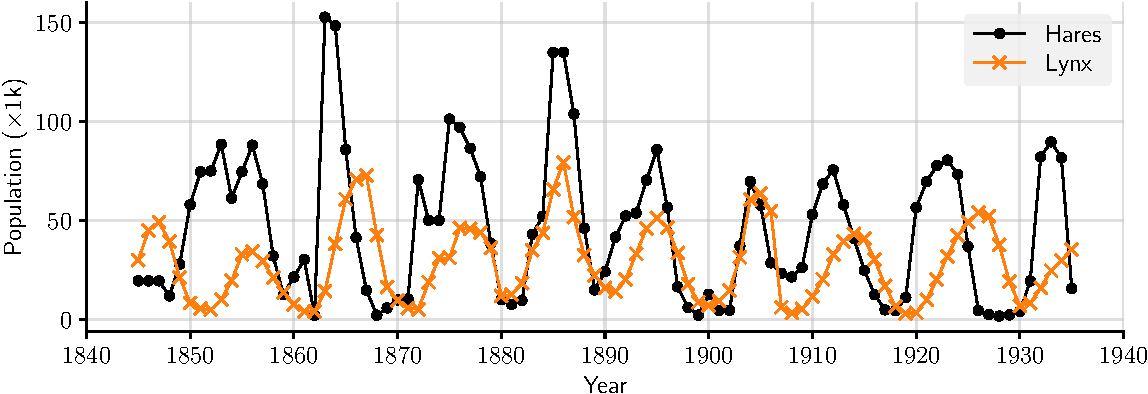
\includegraphics[width=4cm]{\gp{nps/translation_equivariance/data.pdf}}};
        \node [right=2cm of data] (pred) {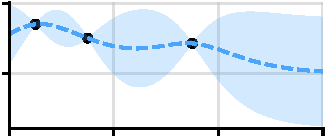
\includegraphics[width=4cm]{\gp{nps/translation_equivariance/pred.pdf}}};
        \draw [arrow, ->] (data) -- node [above, midway] {$\pi$} (pred);
        \node [below=0.75cm of data] (datashifted) {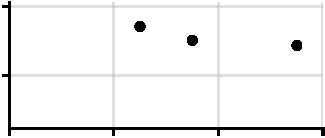
\includegraphics[width=4cm]{\gp{nps/translation_equivariance/data_shifted.pdf}}};
        \draw [arrow, ->] (data) -- node [anchor=west] {$\T_\tau$} (datashifted);
        \node [right=2cm of datashifted] (predshifted) {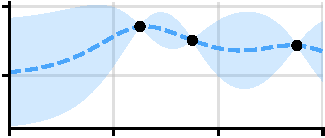
\includegraphics[width=4cm]{\gp{nps/translation_equivariance/pred_shifted.pdf}}};
        \draw [arrow, ->] (datashifted) -- node [above, midway] {$\pi$} (predshifted);
        \draw [arrow, ->] (pred) -- node [anchor=west] {$\T_\tau$} (predshifted);
    \end{tikzpicture}
    \caption[
        Commutative diagram illustrating translation equivariance
    ]{
        Commutative diagram illustrating translation equivariance of a neural process $\pi \colon \D \to \Pc$.
        The predictions of the neural process $\pi$ are shown in dashed blue.
    }
    \label{fig:translation_equivariance}
\end{figure}

\vspace{-0.5em}
Intuitively, if a map is translation equivariant, then, whenever the input is translated, the output is translated similarly.
In the case of a neural process, translation equivariance is illustrated in \cref{fig:translation_equivariance}.
In this case, the map $\pi_\theta \colon \D \to \Qc$ is from data sets $\D$ to stochastic processes $\Qc$.
Translation equivariance then means that, whenever a data set $D$ is shifted by some amount, $\T_\tau D$,
the corresponding prediction $\pi(\T_\tau D)$ is equal to the original prediction, $\pi(D)$, shifted by the same amount, $\T_\tau \pi(D)$.
\pagebreak
Technically, one says that application of the neural process and translation commute.
Another important example of a translation equivariant map is a convolutional neural network \parencite{Fukushima:1982:Neocognitron_A_Self-Organizing_Neural_Network,LeCun:1989:Backpropagation_Applied_to_Handwritten_Zip}.
If we pass a translated version of an input image to a CNN, then %translation equivariance means that
the CNN produces the original output translated by the same amount.

\index{neural process!convolutional}
\Cref{\xrprefix{sec:convcnps:convcnps}} will propose general parametrisations of prediction maps $\pi_\theta\colon \D \to \Qc$ that are translation equivariant.
We call this class of neural processes \emph{convolutional neural processes} (ConvNPs).
Whereas non-convolutional neural processes are implemented with multi-layer perceptrons,
convolutional neural processes are driven by convolutional neural networks.
Examples of ConvNPs are
the Convolutional Conditional Neural Process \parencite[ConvCNP; \cref{\xrprefix{sec:convcnps:convcnps}};][]{Gordon:2020:Convolutional_Conditional_Neural_Processes},
the Convolutional Gaussian Neural Process \parencite[ConvGNP; \cref{\xrprefix{sec:convcnps:gnp}};][]{Markou:2022:Practical_Conditional_Neural_Processes_for_Tractable},
and the Fully Convolutional Gaussian Neural Process \parencite[FullConvGNP; \cref{\xrprefix{sec:convcnps:gnp}};][]{Bruinsma:2021:The_Gaussian_Neural_Process}.

\begin{figure}[t]
    \centering
    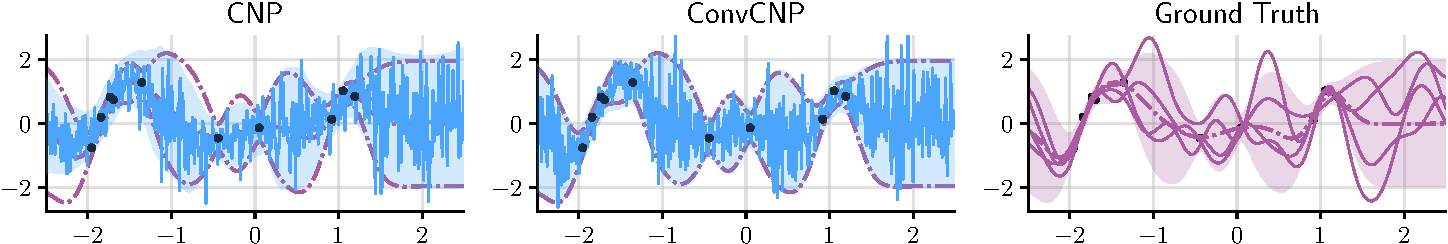
\includegraphics[width=\linewidth]{\gp{nps/te_versus_nonte/plot.pdf}}
    \caption[
        Comparison of a CNP and ConvCNP
    ]{
        Comparison of the prediction of a trained CNP, a non-convolutional neural process, and ConvCNP, a convolutional conditional neural process.
        Shows predictions by the models in dashed blue and predictions by the ground truth in dot-dashed purple.  % Standard
        The models were trained by observing data on $[-2, 2]$.
        We call $[-2, 2]$ the \emph{training range}.
        In the plots, the training range is shaded.
        The left column shows predictions for observations in the training range,
        and the right column shows predictions for observations beyond the training range.
        Filled regions are central 95\%-credible regions.
        The CNP and ConvCNP are taken from the experiment in \cref{\xrprefix{sec:experiments:synthetic}}.
    }
    \label{fig:TE_versus_non-TE}
\end{figure}


\Cref{fig:TE_versus_non-TE}
compares a trained CNP, a non-convolutional neural process,
to a trained ConvCNP, a convolutional neural process.
In the training range (see legend of \cref{fig:TE_versus_non-TE}), the CNP shows a reasonable fit, perhaps slightly underfitting in some places.
However, when it is evaluated outside the training range, the model completely breaks down.
On the other hand, the ConvCNP shows a tight fit, closely recovering the ground truth, and seamlessly generalises to observations beyond the training range.
\looseness=-1
This demonstrates, in a real example, that translation equivariance can improve in-distribution and generalisation performance.

\section{Summary and Outlook}

\Cref{\xrprefix{sec:introduction:overview}} provided a brief outline of this thesis.
Whilst we summarise this chapter, we again connect to future chapters to elucidate the overarching structure in more detail.

A desirable 
probabilistic meta-learning algorithm is one that is \emph{consistent (with respect to the target set)} (\cref{sec:nps:introduction}),
and such a probabilistic meta-learning algorithm can be identified with a \emph{prediction map} (\cref{def:prediction_map}).
This forms the basis for \emph{neural processes}.
A neural process
approaches a meta-learning problem
in a natural way
by directly parametrising a prediction map using neural networks (\cref{sec:nps:neural_processes}).
Compared to stochastic process models such as Gaussian processes, neural processes the circumvent computational challenges associated with computing Bayes' rule by giving up \emph{consistency with respect to the context set} (\cref{sec:nps:consistency}).
In \cref{\xrprefix{chap:predmap}}, we will build on the idea of prediction maps to engage in a rigorous theoretical analysis of neural processes.

To parametrise a prediction map, neural processes often use \emph{encoder--decoder architectures} (\cref{sec:nps:anatomy}).
Although using encoder--decoder architectures is not a necessity, they are a helpful mental model.
In \Cref{\xrprefix{chap:repr_theorems}}, we will study \emph{representation theorems}.
In the context of neural processes, representation theorems are general characterisations of functions on data sets.
Representation theorems can be used to 
theoretically motivate encoder--decoder architectures.

One of the main contributions of this thesis is to build \emph{translation equivariance} (\cref{def:translation_equivariance}) into a neural process (\cref{sec:nps:translation_equivariance}).
For spatial, temporal, and spatio--temporal meta-learning problems, translation-equivariant neural processes can make a better trade-off between flexibility and parameter efficiency.
In \cref{\xrprefix{chap:convcnps}}, we will use the representation theorems from \cref{\xrprefix{chap:repr_theorems}} to construct translation-equivariant neural processes.
We call this class \emph{convolutional neural processes} (ConvNPs).
In addition to ConvNPs,
\cref{\xrprefix{chap:convcnps}} will also introduce the classes of \emph{Gaussian neural processes} (GNPs)
and \emph{autoregressive conditional neural processes} (AR CNPs).
GNPs have the unique ability to model dependencies between target outputs without requiring approximations for the neural process objective.
AR CNPs, which we did not discuss in this chapter, trade the desirable property of consistency for better performance.
Hence, AR CNPs are no longer consistent probabilistic meta-learning algorithms, but they may offer improved predictions.
\looseness=-1
In \cref{\xrprefix{chap:experiments}}, we will put these new models and existing approaches to the test, establishing general weaknesses and strengths.

Over the course of this chapter, one might have noticed that there are \emph{many} flavours of neural processes.
To help with the implementation of all of these flavours,
\cref{\xrprefix{chap:software}} will present a software abstraction that enables the user to rapidly explore neural processes models by putting together elementary building blocks in different ways.















\end{document}



